\documentclass{article}
\usepackage[utf8]{inputenc}
% are all of these packages really necessary?
% no.
% i'm just too lazy to only grab the packages i want for a specific
% document, so i just glob all of my most commonly used packages together
% this is bad practice.
\usepackage{amsmath,amsthm,amssymb,amsfonts, fancyhdr, color, comment, graphicx, environ, mdframed, soul, calc, enumitem, mdframed, xcolor, geometry, empheq, mathtools, tikz, pgfplots, caption, subcaption, hyperref}

\usetikzlibrary{external}
\tikzexternalize[prefix=tikz/,optimize command away=\includepdf]

%tikzpicture
\usepackage{tikz}
\usepackage{scalerel}
\usepackage{pict2e}
\usepackage{tkz-euclide}
\usetikzlibrary{calc}
\usetikzlibrary{patterns,arrows.meta}
\usetikzlibrary{shadows}
\usetikzlibrary{external}

%pgfplots
\usepackage{pgfplots}
\pgfplotsset{compat=newest}
\usepgfplotslibrary{statistics}
\usepgfplotslibrary{fillbetween}
\usepgfplotslibrary{polar}

\tikzset{external/export=true}
\pgfplotsset{
    standard/.style={
    axis line style = thick,
    trig format=rad,
    enlargelimits,
    axis x line=middle,
    axis y line=middle,
    enlarge x limits=0.15,
    enlarge y limits=0.15,
    every axis x label/.style={at={(current axis.right of origin)},anchor=north west},
    every axis y label/.style={at={(current axis.above origin)},anchor=south east}
    }
}
\newcommand*\widefbox[1]{\fbox{\hspace{2em}#1\hspace{2em}}}
% Command "alignedbox{}{}" for a box within an align environment
% Source: http://www.latex-community.org/forum/viewtopic.php?f=46&t=8144
\newlength\dlf  % Define a new measure, dlf
\newcommand\alignedbox[2]{
% Argument #1 = before & if there were no box (lhs)
% Argument #2 = after & if there were no box (rhs)
&  % Alignment sign of the line
{
\settowidth\dlf{$\displaystyle #1$}  
    % The width of \dlf is the width of the lhs, with a displaystyle font
\addtolength\dlf{\fboxsep+\fboxrule}  
    % Add to it the distance to the box, and the width of the line of the box
\hspace{-\dlf}  
    % Move everything dlf units to the left, so that & #1 #2 is aligned under #1 & #2
\boxed{#1 #2}
    % Put a box around lhs and rhs
}
}

\hypersetup{
    colorlinks=true,
    linkcolor=blue,
    filecolor=magenta,      
    urlcolor=cyan,
    pdftitle={Homework 17 Solutions},
    pdfpagemode=UseOutlines,
    bookmarksopen=true,
    pdfauthor={Christina Phan}
}
\newcommand{\lrp}[1]{\left( #1 \right)}
\newcommand{\abs}[1]{\left\vert #1 \right\vert}
\newcommand{\lra}[1]{\left\langle #1 \right\rangle}
\newcommand{\lrb}[1]{\left[ #1 \right]}
\newcommand{\norm}[1]{\left\lVert #1 \right\rVert}
\newcommand{\iintR}[0]{\iint\limits_{R}}
\renewcommand{\u}[0]{\mathbf{u}}
\renewcommand{\i}[0]{\mathbf{i}}
\renewcommand{\j}[0]{\mathbf{j}}
\renewcommand{\k}[0]{\mathbf{k}}
\newcommand{\T}[0]{\mathbf{T}}
\newcommand{\N}[0]{\mathbf{N}}
\newcommand{\B}[0]{\mathbf{B}}
\renewcommand{\r}[0]{\mathbf{r}}
\renewcommand{\a}[0]{\mathbf{a}}
\renewcommand{\v}[0]{\mathbf{v}}
\newcommand{\F}[0]{\mathbf{F}}
\newcommand{\eqq}[0]{\stackrel{?}{=}}

\geometry{letterpaper, portrait, margin=1in}
\renewcommand{\footrulewidth}{0.8pt}
\setlength\parindent{0pt}
\pagestyle{fancy}
\lhead{Christina Phan}
\rhead{MAT 21D} 
\chead{\textbf{Homework 17 Solutions}}

\newcommand{\Solution}{\textit{Solution}}
\pgfplotsset{compat=1.18}
\begin{document}

\phantomsection
\addcontentsline{toc}{section}{Problem 1 (Parts)}\textbf{Problem 1 (Parts)}

Find a parameterization $\r(u,v)$ of the surface that is defined over a rectangle in the $uv$-plane (that is, you should have bounds of the form $a\leq u\leq b$, $c\leq v\leq d$):

\phantomsection
\addcontentsline{toc}{subsection}{1(a)}\textbf{(a)} The paraboloid $z=9-x^2-y^2$, $z\geq 0$

\Solution

Let's rewrite this paraboloid a little bit.
\begin{equation*}
    z=9-(x^2+y^2)
\end{equation*}
The $x^2+y^2$ really reminds me of cylindrical coordinates...

Let's use cylindrical coordinates!

Recall that in cylindrical coordinates,
\begin{align*}
    x&=r\cos \theta\\
    y&=r\sin \theta\\
    z&=z
\end{align*}
Now, we know what $x$ and $y$ are in terms of $r$ and $\theta$.

We just need to find out what $z$ is in terms of $r$ and $\theta$.

Using our paraboloid equation,
\begin{align*}
    z&=9-(x^2+y^2)\\
    z&=9-(r^2)\tag{in polar, $x^2+y^2=r^2$}\\
    z&=9-r^2
\end{align*}
In terms of $r$ and $\theta$, our $x$, $y$, and $z$ values are
\begin{align*}
    x&=r\cos \theta\\
    y&=r\sin \theta\\
    z&=9-r^2
\end{align*}
Let's find the bounds for $r$ and $\theta$.

For $r$,

Since $z\leq 0$,
\begin{align*}
    9-r^2&\geq 0\\
    9 &\geq r^2\\
    3&\geq r\tag{$r\geq 0$ is always true}
\end{align*}

For $\theta$,

Since we're going around the entire paraboloid, our our lower and upper bounds for $\theta$ are $\theta=0$ and $\theta=2\pi$, respectively.

Our final answer is
\begin{equation*}
    \boxed{\r(r,\theta)=\lra{r\cos \theta, r\sin\theta, 9-r^2}}\tag{$0\leq r\leq 3$, $0\leq \theta\leq 2\pi$}
\end{equation*}
\phantomsection
\addcontentsline{toc}{subsection}{1(b)}\textbf{(b)} The portion of the cone $z=2\sqrt{x^2+y^2}$ between the planes $z=2$ and $z=4$

\Solution

The $x^2+y^2$ really reminds me of polar (cylindrical) coordinates...

Let's use cylindrical coordinates!

Recall that in cylindrical coordinates,
\begin{align*}
    x&=r\cos \theta\\
    y&-r\sin\theta\\
    z&=z
\end{align*}
Now, we know what $x$ and $y$ are in terms of $r$ and $\theta$.

We just need to find out what $z$ is in term of $r$ and $\theta$.

Using our cone equation,
\begin{align*}
    z&=2\sqrt{x^2+y^2}\\
    &=2\sqrt{r^2}\tag{in polar, $x^2+y^2=r^2$}\\
    &=2r\tag{$r\geq 0$ is always true}
\end{align*}
In terms of $r$ and $\theta$, our $x$, $y$, and $z$ values are
\begin{align*}
    x&=r\cos\theta\\
    y&=r\sin\theta\\
    z&=2r
\end{align*}
Let's find the bounds for $r$ and $\theta$.

For $r$,

Since $2\leq z\leq 4$,
\begin{align*}
    2\leq &2r\leq 4\\
    1\leq & r\leq 2
\end{align*}

For $\theta$,

Since we're going around the entire cone, our lower and upper bounds for $\theta$ are $\theta=0$ and $\theta=2\pi$, respectively.

Our final answer is
\begin{equation*}
    \boxed{\r(r,\theta)=\lra{r\cos \theta, r\sin \theta, 2r}}\tag{$1\leq r\leq 2$, $0\leq \theta\leq 2\pi$}
\end{equation*}
\phantomsection
\addcontentsline{toc}{subsection}{1(c)}\textbf{(c)} The portion of the sphere $x^2+y^2+z^2=4$ in the first octant between the $xy$-plane
and the cone $z=\sqrt{x^2+y^2}$

\Solution

Since we're only in the first octant, the sphere's $x^2+y^2+z^2=4$ is really just
\begin{align*}
    z^2&=4-x^2-y^2\\
    z^2&=4-(x^2+y^2)\\
    z&=\sqrt{4-(x^2+y^2)}\tag{first octant only}
\end{align*}
The $x^2+y^2$ really reminds me of cylindrical coordinates...

Let's use cylindrical coordinates!

Recall that in cylindrical coordinates,
\begin{align*}
    x&=r\cos \theta\\
    y&=r\sin \theta\\
    z&=z
\end{align*}
Now, we know what $x$ and $y$ are in terms of $r$ and $\theta$.

We just need to find out what $z$ is in terms of $r$ and $\theta$.

Using our rewritten sphere equation,
\begin{align*}
  z&=\sqrt{4-(x^2+y^2)}\\
  z&=\sqrt{4-(r^2)}\tag{in polar, $x^2+y^2=r^2$}\\
  z&=\sqrt{4-r^2}
\end{align*}
In terms of $r$ and $\theta$, our $x$, $y$, and $z$ values are
\begin{align*}
    x&=r\cos\theta\\
    y&=r\sin\theta\\
    z&=\sqrt{4-r^2}
\end{align*}
Let's find the bounds for $r$ and $\theta$.

For $r$,

We know $z$ is  bounded above by $z=\sqrt{4-(x^2+y^2}$ (sphere) and below by $z=\sqrt{x^2+y^2}$ (cone). The upper bound of $r$ is going to come from the sphere. If we find where the sphere and cone intersect, we can find the lower bound of $r$.

For the lower bound,
\begin{align*}
    x^2+y^2+z^2&=4\\
    x^2+y^2+\lrp{\sqrt{x^2+y^2}}^2&=\\
    x^2+y^2+\lrp{x^2+y^2}&=\\
    2x^2+2y^2&=\\
    x^2+y^2&=2\\
    r^2&=2\tag{in polar, $x^2+y^2=r^2$}\\
    r&=\sqrt{2}\tag{$r\geq 0$ is always true}
\end{align*}
For the upper bound,

When $z=0$
\begin{align*}
    0&=\sqrt{4-r^2}\\
    0&=4-r^2\\
    r^2&=4\\
    r&=2\tag{$r\geq 0$ is always true}
\end{align*}
Therefore, our lower and upper bounds for $r$ are $r=\sqrt{2}$ and $r=2$, respectively.

For $\theta$,

Since we're \textit{only} in the first octant, $0\leq \theta\leq \dfrac{\pi}{2}$ (draw a circle and see which angles bound \textit{just} the first quadrant).

Our final answer is
\begin{equation*}
    \boxed{\r(r,\theta)=\lra{r\cos\theta, r\sin\theta, \sqrt{4-r^2}}}\tag{$\sqrt{2}\leq r\leq 2$, $0\leq \theta\leq \dfrac{\pi}{2}$}
\end{equation*}
\phantomsection
\addcontentsline{toc}{subsection}{1(d)}\textbf{(d)} The surface cut from the parabolic cylinder $z=4-y^2$ by the planes $x=0$, $x=2$, and $z=0$

\Solution

Cylindrical and spherical coordinates might not work out for us here...

Instead, let's have $\r$ be a function in terms of $x$ and $y$. With this parameterization in mind,
\begin{align*}
    x&=x\\
    y&=y\\
    z&=f(x,y)
\end{align*}
Now, we know what $x$ and $y$ are in terms of $x$ and $y$.

We just need to find out what $z$ is in terms of $x$ and $y$.

Using our parabolic cylinder equation, we know $z=4-y^2$.

In terms of $x$ and $y$, our $x$, $y$, and $z$ values are
\begin{align*}
    x&=x\\
    y&=y\\
    z&=4-y^2
\end{align*}
Let's find the bounds for $x$ and $y$.

For $x$,

Our problem tells us that we're bounded below by $x=0$ and above by $x=2$.

For $y$,

Our problem tells us we're bounded by $z=0$. 

From our parabolic cylinder equation,
\begin{align*}
    0&=4-y^2\\
    y^2&=4\\
    y&=\pm 2
\end{align*}
Therefore, we're bounded below by $y=2$ and above by $y=2$.

Our final answer is
\begin{equation*}
    \boxed{\r(x,y)=\lra{x,y,4-y^2}}\tag{$0\leq x\leq 2$, $-2\leq y\leq 2$}
\end{equation*}

\phantomsection
\addcontentsline{toc}{subsection}{1(e)}\textbf{(e)} The portion of the cylinder $x^2+z^2=4$ above the $xy$-plane between the planes $y=-2$ and $y=2$

\Solution

The $x^2+z^2$ really reminds me of cylindrical coordinates...

Let's (kind of) use cylindrical coordinates!

Instead of the standard $x=r\cos\theta$, $y=r\sin\theta$, let's have
\begin{align*}
    x&=r\cos \theta\\
    y&=y\\
    z&=r\sin \theta
\end{align*}
Since $x^2+z^2=4$, we know $r^2=4$ which means $r=2$.

Therefore,
\begin{align*}
    x&=2\cos\theta\\
    y&=y\\
    z&=2\sin\theta
\end{align*}
Now, we know what $x$ and $z$ are in terms of $\theta$.

We can have $y$ be our other unknown variable.

Let's find the bounds for $y$ and $\theta$.

For $y$,

Our problem tells us that we're bounded below by $y=-2$ and above by $y=2$.

For $\theta$,

Since we're going \textit{above} the $xy$-plane ($z\geq 0$), $0\leq \theta\leq \pi$. Graphically, this makes sense. If we draw a unit circle where $x=\cos \theta$ and $z=\sin\theta$, we get
\begin{center}
\resizebox{4cm}{!}{
    \begin{tikzpicture}
    \begin{axis}[standard,
            xtick={-2.718,2.718},
            ytick={-2.718,2.718},
            samples=1000,
            xlabel={$x$},
            ylabel={$z$},
            xmin=-3,xmax=3,
            ymin=-3,ymax=3,
            x=1cm,
            y=1cm/1,
            xticklabels={$-1$,$1$},
            yticklabels={$-1$,$1$}
           ]
\node[anchor=center,label=south west:$O$] at (axis cs:0,0){};
\addplot[name path=F,domain={-2.718:2.718}]{sqrt(2.718^2-x^2};
\addplot[name path=G,domain={-2.718:2.718}]{-sqrt(2.718^2-x^2};
\addplot[name path=H,domain={-2.718:2.718}]{0};
    \end{axis}
    \end{tikzpicture}
}
\end{center}
Again, we just want the portion \textit{above} the $xy$-plane ($z\geq 0$), so our angle $\theta$ must be in between $\theta=0$ and $\theta=\pi$.

Our final answer is
\begin{equation*}
    \boxed{\r(y,\theta)=\lra{2\cos\theta, y,2\sin\theta}}\tag{$-2\leq y\leq 2$, $0\leq \theta\leq \pi$}
\end{equation*}

\phantomsection
\addcontentsline{toc}{subsection}{1(f)}\textbf{(f)} The portion of the plane $x + y + z = 1$ inside the cylinder $y^2+z^2=9$

\Solution

The $y^2+z^2$ really reminds me of cylindrical coordinates...

Let's (kind of) use cylindrical coordinates!

Instead of the standard $x=r\cos\theta$, $y=r\sin\theta$, let's have
\begin{align*}
    x&=x\\
    y&=r\cos\theta\\
    z&=r\sin\theta
\end{align*}
Now, we know what $y$ and $z$ are in terms of $r$ and $\theta$.

We just need to find out what $x$ is in terms of $r$ and $\theta$.

Using our plane equation,
\begin{align*}
    x+y+z&=1\\
    x&=1-y-z\\
    x&=1-r\cos\theta-r\sin\theta
\end{align*}
In terms of $r$ and $\theta$, our $x$, $y$, and $z$ values are
\begin{align*}
    x&=1-r\cos\theta-r\sin\theta\\
    y&=r\cos\theta\\
    z&=r\sin\theta
\end{align*}
Let's find the bounds for $r$ and $\theta$.

For $r$,

Since $y^2+z^2\leq 9$ (we're inside the cylinder), we know $r^2\leq 9$
 which means $0\leq r\leq 3$ ($r\geq 0$ is always true).
 
For $\theta$,

Since we're going around the entire cylinder, $0\leq \theta\leq 2\pi$.

Our final answer is
\begin{align*}
    \boxed{\r(r,\theta)\lra{1-r\cos\theta-r\sin\theta,r\cos\theta,r\sin\theta}}\tag{$0\leq r\leq 3$, $0\leq \theta\leq 2\pi$}
\end{align*}
 
\phantomsection
\addcontentsline{toc}{section}{Problem 2 (Parts)}\textbf{Problem 2 (Parts)}

Use a parametrization to find the area of the surface:

\phantomsection
\addcontentsline{toc}{subsection}{2(a)}\textbf{(a)} The portion of the plane $y+2z=2$ inside the cylinder $x^2+y^2=1$

\Solution

\phantomsection
\addcontentsline{toc}{subsubsection}{Parametrization}
\textbf{Parametrization}

Let's find our parametrization of the surface.

The $x^2+y^2$ really reminds of cylindrical coordinates.

Let's use cylindrical coordinates!

Recall that in cylindrical coordiantes,
\begin{align*}
    x&=r\cos\theta\\
    y&=r\sin\theta\\
    z&=z
\end{align*}
Now, we know what $x$ and $y$ are in terms of $r$ and $\theta$.

We just need to find out what $z$ is in terms of $r$ and $\theta$.

Using our plane equation,
\begin{align*}
    y+2z&=2\\
    2z&=2-y\\
    z&=1-\frac{1}{2}y\\
    z&=1-\frac{1}{2}r\sin\theta
\end{align*}
In terms of $r$ and $\theta$, our $x$, $y$, and $z$ values are
\begin{align*}
    x&=r\cos\theta\\
    y&=r\sin\theta\\
    z&=1-\frac{1}{2}r\sin\theta
\end{align*}
Let's find the bounds for $r$ and 
$\theta$.

For $r$,

Since we're \textit{inside} the cylinder $x^2+y^2=1$,
\begin{align*}
    x^2+y^2&\leq 1\\
    r^2&\leq 1\tag{in polar, $x^2+y^2=r^2$}\\
    r&\leq 1\tag{$r\geq 0$ is always true}
\end{align*}

For $\theta$,

Since we're going around the entire cylinder, $0\leq \theta\leq 2\pi$.

Therefore, our parameterization is
\begin{equation*}
    \r(r,\theta)=\lra{r\cos\theta,r\sin\theta, 1-\frac{1}{2}r\sin\theta}\tag{$0\leq r\leq 1$, $0\leq \theta\leq 2\pi$}
\end{equation*}
\phantomsection
\addcontentsline{toc}{subsubsection}{Surface Area}\textbf{Surface Area}

Now that we have our parameterization, let's calculate the surface area.

Recall that the surface area is
\begin{align*}
    S&=\iint_R \norm{\frac{\partial \r}{\partial u}\times \frac{\partial \r}{\partial v}}\,dA
\end{align*}
Let's have $u=r$ and $v=\theta$.

We know our region is $0\leq r\leq 1$ and $0\leq \theta\leq 2\pi$.

Let's find what $\displaystyle\norm{\frac{\partial \r}{\partial r}\times \frac{\partial \r}{\partial \theta}} $ is.

Since $\displaystyle\r(r,\theta)=\lra{r\cos\theta,r\sin\theta, 1-\frac{1}{2}r\sin\theta}$
\begin{align*}
    \frac{\partial \r}{\partial r}&=\lra{\cos\theta, \sin\theta, -\frac{1}{2}\sin\theta}\\
    \frac{\partial \r}{\partial \theta}&=\lra{-r\sin\theta, r\cos\theta, -\frac{1}{2}r\cos\theta}\\
    \frac{\partial \r}{\partial r}\times \frac{\partial \r}{\partial \theta}&=\begin{vmatrix}
\mathbf{i} & \mathbf{j} & \mathbf{k}\\
\cos\theta & \sin\theta & -\frac{1}{2}\sin\theta\\
-r\sin\theta & r\cos\theta & -\frac{1}{2}r\cos\theta\\
\end{vmatrix}\\
&=\lrp{-\frac{1}{2}r\sin\theta\cos\theta+\frac{1}{2}r\sin\theta\cos\theta}\i -\lrp{-\frac{1}{2}r\cos^2\theta - \frac{1}{2}r\sin^2\theta}\j + \lrp{r\cos^2\theta + r\sin^2\theta}\k\\
&=\lrp{0}\i -\Bigg(-\frac{1}{2}r\lrp{\cos^2\theta+\sin^2\theta}\Bigg)\j+\Big(r(\cos^2\theta+\sin^2\theta\Big)\k\\
&=0\i -\lrp{-\frac{1}{2}r}\j+\lrp{r}\k\tag{$\cos^2\theta+\sin^2\theta=1$}\\
&=0\i +{\frac{1}{2}r}\j+r\k\\
&=\lra{0, \frac{1}{2}r,r}\\
\norm{\frac{\partial \r}{\partial r}\times \frac{\partial \r}{\partial \theta}}&=\sqrt{0^2+\lrp{\frac{1}{2}r}^2+r^2}=\sqrt{\frac{1}{4}r^2+r^2}=\sqrt{\frac{5}{4}r^2}=\frac{\sqrt{5}}{2}r
\end{align*}
Let's evaluate the integral.
\begin{align*}
    S&=\int_0^{2\pi}\int_0^1 \frac{\sqrt{5}}{2}r\,dr\,d\theta\\
    &=\int_0^{2\pi}\lrb{\frac{\sqrt{5}}{4}r^2}_0^1\,d\theta\\
    &=\int_0^{2\pi}\frac{\sqrt{5}}{4}\,d\theta\\
    &=\lrb{\frac{\sqrt{5}}{4}\theta}_0^{2\pi}\\
    &=\frac{\sqrt{5}}{4}\lrp{2\pi}\\
    &=\boxed{\frac{\sqrt{5}}{2}\pi}
\end{align*}
\phantomsection
\addcontentsline{toc}{subsection}{2(b)} \textbf{(b)} The portion of the cone $\displaystyle z=\frac{1}{3}\sqrt{x^2+y^2}$ between the planes $z=1$ and $z= \frac{4}{3}$

\Solution

\phantomsection
\addcontentsline{toc}{subsubsection}{Parametrization}\textbf{Parametrization}

Let's find our parametrization of the surface.

The $x^2+y^2$ really reminds me of cylindrical coordinates...

Let's use cylindrical coordinates!

Recall that in cylindrical coordinates
\begin{align*}
    x&=r\cos\theta\\
    y&=r\sin\theta\\
    z&=z
\end{align*}
Now, we know what $x$ and $y$ are in terms of $r$ and $\theta$.

We just need to find out what $z$ is in terms of $r$ and $\theta$.

Using our cone equation,
\begin{align*}
    z&=\frac{1}{3}\sqrt{x^2+y^2}\\
    &=\frac{1}{3}\sqrt{r^2}\tag{in polar, $x^2+y^2=r^2$}\\
    &=\frac{1}{3}r\tag{$r\geq 0$ is always true}
\end{align*}
In terms of $r$ and $\theta$, our $x$, $y$, and $z$ values are
\begin{align*}
    x&=r\cos\theta\\
    y&=r\sin\theta\\
    z&=\frac{1}{3}r
\end{align*}
Let's find the bounds for $r$ and $\theta$.

For $r$,

Our problem tells us that we're bounded below by $z=1$ and above by $z=\frac{4}{3}$.

Therefore,
\begin{align*}
    1\leq&z\leq \frac{4}{3}\\
    \implies 1\leq &\frac{1}{3}r\leq \frac{4}{3}\\
    3\leq &r \leq 4
\end{align*}

For $\theta$,

Since we're going around he entire cone, $0\leq \theta\leq 2\pi$.

Therefore, our parameterization is
\begin{equation*}
    \r(r,\theta)=\lra{r\cos\theta, r\sin\theta, \frac{1}{3}r}\tag{$3\leq r\leq 4$, $0\leq \theta\leq 2\pi$}
\end{equation*}
\phantomsection
\addcontentsline{toc}{subsubsection}{Surface Area}\textbf{Surface Area}

Now that we have our parameterization, let's calculate the surface area.

Recall that the surface area is
\begin{align*}
    S&=\iint_R \norm{\frac{\partial \r}{\partial u}\times \frac{\partial \r}{\partial v}}\,dA
\end{align*}
Let's have $u=r$ and $v=\theta$.

We know our region is $3\leq r\leq 4$ and $0\leq \theta\leq 2\pi$.

Let's find what $\displaystyle\norm{\frac{\partial \r}{\partial r}\times \frac{\partial \r}{\partial \theta}} $ is.

Since $\displaystyle \r(r,\theta)=\lra{r\cos\theta, r\sin\theta, \frac{1}{3}r}$,
\begin{align*}
    \frac{\partial \r}{\partial r}&=\lra{\cos\theta, \sin\theta, \frac{1}{3}}\\
    \frac{\partial \r}{\partial \theta}&=\lra{-r\sin\theta, r\cos\theta, 0}\\
    \frac{\partial \r}{\partial r}\times \frac{\partial \r}{\partial \theta}&=\begin{vmatrix}
\mathbf{i} & \mathbf{j} & \mathbf{k}\\
\cos\theta & \sin\theta & \frac{1}{3}\\
-r\sin\theta& r\cos\theta & 0\\
\end{vmatrix}\\
&=\lrp{0-\frac{1}{3}r\cos\theta}\i -\lrp{0+\frac{1}{3}r\sin\theta}\j+\lrp{r\cos^2\theta+r\sin^2\theta}\k\\
&=\lrp{-\frac{1}{3}r\cos\theta}+\lrp{\frac{1}{3}r\sin\theta}\j+\Big(r\lrp{\cos^2\theta+\sin^2\theta}\Big)\k\\
&=\lrp{-\frac{1}{3}r\cos\theta}+\lrp{\frac{1}{3}r\sin\theta}\j+\lrp{r}\k\tag{$\cos^2\theta+\sin^2\theta=1$}\\
&=\lra{-\frac{1}{3}r\cos\theta,\frac{1}{3}r\sin\theta,r}\\
\norm{\frac{\partial \r}{\partial r}\times \frac{\partial \r}{\partial \theta}}&=\sqrt{\lrp{-\frac{1}{3}r\cos\theta}^2+\lrp{\frac{1}{3}r\sin\theta}+r^2}\\
&=\sqrt{\frac{1}{9}r^2\cos^2\theta+\frac{1}{9}r^2\sin^2\theta+r^2}\\
&=\sqrt{\frac{1}{9}r^2\lrp{\cos^2\theta+\sin^2\theta}+r^2}\\
&=\sqrt{\frac{1}{9}r^2+r^2}\tag{$\cos^2\theta+\sin^2\theta=1$}\\
&=\sqrt{\frac{10}{9}r^2}\\
&=\frac{\sqrt{10}}{3}r
\end{align*}
Let's evaluate the integral.
\begin{align*}
    S&=\int_0^{2\pi}\int_3^4\frac{\sqrt{10}}{3}r\,dr\,d\theta\\
    &=\int_0^{2\pi}\lrb{\frac{\sqrt{10}}{6}r^2}_3^4\,d\theta\\
    &=\int_0^{2\pi}\frac{\sqrt{10}}{6}(4)^2-\frac{\sqrt{10}}{6}(3)^2\,d\theta\\
    &=\int_0^{2\pi}\frac{7\sqrt{10}}{6}\,d\theta\tag{use a calculator}\\
    &=\lrb{\frac{7\sqrt{10}}{6}\theta}_0^{2\pi}\\
    &=\frac{7\sqrt{10}}{6}\lrp{2\pi}\\
    &=\boxed{\frac{7\sqrt{10}}{3}}
\end{align*}
\phantomsection
\addcontentsline{toc}{subsection}{2(c)}\textbf{(c)} The portion of the paraboloid $z=x^2+y^2$ between the planes $z=1$ and $z=4$

\Solution

\phantomsection
\addcontentsline{toc}{subsubsection}{Parametrization}\textbf{Parametrization}

Let's find our parametrization of the surface.

The $x^2+y^2$ really reminds me of cylindrical coordinates...

Let's use cylindrical coordinates!

Recall that in cylindrical coordinates
\begin{align*}
    x&=r\cos\theta\\
    y&=r\sin\theta\\
    z&=z
\end{align*}
Now, we know what $x$ and $y$ are in terms of $r$ and $\theta$.

We just need to find out what $z$ is in terms of $r$ and $\theta$.

Using our paraboloid equation,
\begin{align*}
    z&=x^2+y^2\\
    z&=r^2\tag{in polar, $x^2+y^2=1$}
\end{align*}
In terms of $r$ and $\theta$, our $x$, $y$, and $z$ values are
\begin{align*}
    x&=r\cos\theta\\
    y&=r\sin\theta\\
    z&=r^2
\end{align*}
Let's find the bounds for $r$ and $\theta$.

For $r$,

Since we're between the planes $z=1$ and $z=4$,
\begin{align*}
    1\leq&z\leq 4\\
    \implies 1\leq &r^2\leq 4\\
    1\leq &r\leq 2\tag{$r\geq 0$ is always true}
\end{align*}

For $\theta$,

Since we're going around the entire cone, $0\leq \theta\leq 2\pi$.

Therefore, our parameterization is
\begin{equation*}
    \r(r,\theta)=\lra{r\cos\theta, r\sin\theta, r^2}\tag{$1\leq r\leq 2$, $0\leq \theta\leq 2\pi$}
\end{equation*}
\phantomsection
\addcontentsline{toc}{subsubsection}{Surface Area}\textbf{Surface Area}

Now that we have our parameterization, let's calculate the surface area.

Recall that the surface area is
\begin{align*}
    S&=\iint_R \norm{\frac{\partial \r}{\partial u}\times \frac{\partial \r}{\partial v}}\,dA
\end{align*}
Let's have $u=r$ and $v=\theta$.

We know our region is $1\leq r\leq 2$ and $0\leq \theta\leq 2\pi$.

Let's find what $\displaystyle\norm{\frac{\partial \r}{\partial r}\times \frac{\partial \r}{\partial \theta}} $ is.

Since $\displaystyle \r(r,\theta)=\lra{r\cos\theta, r\sin\theta, r^2}$,
\begin{align*}
    \frac{\partial \r}{\partial r}&=\lra{\cos\theta, \sin\theta, 2r}\\
    \frac{\partial \r}{\partial \theta}&=\lra{-r\sin\theta, r\cos\theta,0}\\
    \frac{\partial \r}{\partial r}\times \frac{\partial \r}{\partial \theta}&=\begin{vmatrix}
\mathbf{i} & \mathbf{j} & \mathbf{k}\\
\cos\theta & \sin\theta& 2r\\
-r\sin\theta& r\cos\theta & 0\\
\end{vmatrix}\\
&=\lrp{0-2r^2\cos\theta}\i-\lrp{0+2r^2\sin\theta}\j+\lrp{r\cos^2\theta+r\sin^2\theta}\k\\
&=\lrp{-2r^2\cos\theta}\i-\lrp{2r^2\sin\theta}+\Big(r\lrp{\cos^2\theta+\sin^2\theta}\Big)\k\\
&=\lrp{-2r^2\cos\theta}\i-\lrp{2r^2\sin\theta}+\lrp{r}\k\tag{$\cos^2\theta+\sin^2\theta=1$}\\
&=\lra{-2r^2\cos\theta,2r^2\sin\theta,r}\\
\norm{\frac{\partial \r}{\partial u}\times \frac{\partial \r}{\partial v}}&=\sqrt{\lrp{-2r^2\cos\theta}^2+\lrp{2r^2\sin\theta}^2+r^2}\\
&=\sqrt{4r^4\cos^2\theta+4r^4\sin^2\theta+r^2}\\
&=\sqrt{4r^4\lrp{\cos^2\theta+\sin^2\theta}+r^2}\\
&=\sqrt{4r^4+r^2}\tag{$\cos^2\theta+\sin^2\theta=1$}\\
&=\sqrt{r^2\lrp{4r^2+1}}\\
&=r\sqrt{4r^2+1}\tag{$r\geq 0$ is always true}
\end{align*}
Let's evaluate the integral.
\begin{align*}
    S&=\int_0^{2\pi}\int_1^2 r\sqrt{4r^2+1}\,dr\,d\theta\\
    &u=4r^2+1\hspace{2em}du=8r\,dr\\
    &u(1)=5\hspace{2em}u(2)=17\\
    &=\int_0^{2\pi}\int_5^9 \frac{1}{8}\sqrt{u}\,du\,d\theta\\
    &=\int_0^{2\pi}\lrb{\frac{1}{12}u^{3/2}}_5^{17}\,d\theta\\
    &=\int_0^{2\pi}\lrp{\frac{17^{3/2}-5^{3/2}}{12}}\,d\theta\\
    &=\lrb{\frac{17^{3/2}-5^{3/2}}{12}\theta}_0^{2\pi}\\
    &=\lrp{\frac{17^{3/2}-5^{3/2}}{12}}\lrp{2\pi}\\
    &=\boxed{\frac{17^{3/2}-5^{3/2}}{6}\pi}
\end{align*}

\phantomsection
\addcontentsline{toc}{subsection}{2(d)}\textbf{(d)} The cap cut from the paraboloid $z=2-x^2-y^2$ by the cone $z=\sqrt{x^2+y^2}$

\Solution

\phantomsection
\addcontentsline{toc}{subsubsection}{Parametrization}\textbf{Parametrization}

Let's find our parametrization of the surface.

Let's rewrite our paraboloid equation.
\begin{equation*}
    z=2-x^2-y^2=2-(x^2+y^2)
\end{equation*}

The $x^2+y^2$ really reminds me of cylindrical coordinates...

Let's use cylindrical coordinates!

Recall that in cylindrical coordinates
\begin{align*}
    x&=r\cos\theta\\
    y&=r\sin\theta\\
    z&=z
\end{align*}
Now, we know what $x$ and $y$ are in terms of $r$ and $\theta$.

We just need to find out what $z$ is in terms of $r$ and $\theta$.

Using our rewritten paraboloid equation,
\begin{align*}
    z&=2-(x^2+y^2)\\
    z&=2-r^2\tag{in polar, $x^2+y^2=1$}
\end{align*}
In terms of $r$ and $\theta$, our $x$, $y$, and $z$ values are
\begin{align*}
    x&=r\cos\theta\\
    y&=r\sin\theta\\
    z&=2-r^2
\end{align*}
Let's find the bounds for $r$ and $\theta$.

For $r$,

We need to find out at what $z$ value do the cap and the cone intersect. That is,
\begin{align*}
   z&= 2-(x^2-y^2)\\
   z&=2-z^2\tag{$z=\sqrt{x^2+y^2}$ from cone}\\
   z^2+z-2&=0\\
   (z-1)(z+2)&=0\\
   z&=1\tag{$z\neq 2$ since $z=\sqrt{x^2+y^2}>0$}
\end{align*}
Therefore, our bounds for $z$ are $z=1$ (the intersection), to $z=2$ (the top of the cap).

Since we're between the planes $z=1$ and $z=2$,
\begin{align*}
    1\leq&z\leq 2\\
    \implies 1\leq &2- r^2\leq 2\\
    -1 \leq & -r^2 \leq 1\\
    1 \leq & r^2 \leq -1\\
    0  \leq &r^2 \leq 1\tag{$r^2\geq 0$ is always true}\\
    0 \leq& r\leq 1\tag{$r\geq 0$ is always true}
\end{align*}
For $\theta$,

Since we're going around the entire cap, $0\leq \theta\leq 2\pi$.

Therefore, our parameterization is
\begin{equation*}
    \r(r,\theta)=\lra{r\cos\theta, r\sin\theta, 2-r^2}\tag{$0\leq r\leq 1$, $0\leq \theta\leq 2\pi$}
\end{equation*}
\phantomsection
\addcontentsline{toc}{subsubsection}{Surface Area}\textbf{Surface Area}

Now that we have our parameterization, let's calculate the surface area.

Recall that the surface area is
\begin{align*}
    S&=\iint_R \norm{\frac{\partial \r}{\partial u}\times \frac{\partial \r}{\partial v}}\,dA
\end{align*}
Let's have $u=r$ and $v=\theta$.

We know our region is $0\leq r\leq 1$ and $0\leq \theta\leq 2\pi$.

Let's find what $\displaystyle\norm{\frac{\partial \r}{\partial r}\times \frac{\partial \r}{\partial \theta}} $ is.

Since $\displaystyle \r(r,\theta)=\lra{r\cos\theta, r\sin\theta, 2-r^2}$,
\begin{align*}
    \frac{\partial \r}{\partial r}&=\lra{\cos\theta,\sin\theta,-2r}\\
    \frac{\partial \r}{\partial \theta}&=\lra{-r\sin\theta, r\cos\theta, 0}\\
    \frac{\partial \r}{\partial r}\times \frac{\partial \r}{\partial \theta}&=\begin{vmatrix}
\mathbf{i} & \mathbf{j} & \mathbf{k}\\
\cos\theta & \sin\theta & -2r\\
-r\sin\theta & r\cos\theta & 0\\
\end{vmatrix}\\
&=\lrp{0+2r^2\cos\theta}\i -\lrp{0-2r^2\sin\theta}\j+\lrp{r\cos^2\theta+r\sin^2\theta}\k\\
&=\lrp{2r^2\cos\theta}\i-\lrp{-2r^2\sin\theta}\j +\Big(r\lrp{\cos^2\theta+\sin^2\theta}\Big)\k\\
&=\lrp{2r^2\cos\theta}\i+\lrp{2r^2\sin\theta}\j+\lrp{r}\k\tag{$\cos^2\theta+\sin^2\theta=1$}\\
&=\lra{2r^2\cos\theta,2r^2\sin\theta,r}\\
\norm{\frac{\partial \r}{\partial r}\times \frac{\partial \r}{\partial \theta}}&=\sqrt{\lrp{2r^2\cos\theta}^2+\lrp{2r^2\sin\theta}^2+r^2}\\
&=\sqrt{4r^4\cos^2\theta+4r^4\sin^2\theta+r^2}\\
&=\sqrt{4r^4\lrp{\cos^2\theta+\sin^2\theta}+r^2}\\
&=\sqrt{4r^4+r^2}\tag{$\cos^2\theta+\sin^2\theta=1$}\\
&=\sqrt{r^2(4r^2+1)}\\
&=r\sqrt{4r^2+1}\tag{$r\geq 0$ is always true}
\end{align*}
Let's evaluate the integral.
\begin{align*}
    S&=\int_0^{2\pi}\int_0^1 r\sqrt{4r^2+1}\,dr\,d\theta\\
    &u=4r^2+1\hspace{2em}du=8r\,dr\\
    &u(0)=1\hspace{2em}u(1)=5\\
    &=\int_0^{2\pi}\int_1^5 \frac{1}{8}\sqrt{u}\,du\,d\theta\\
    &=\int_0^{2\pi}\lrb{\frac{1}{12}u^{3/2}}_1^5\,d\theta\\
    &=\int_0^{2\pi}\lrp{\frac{5^{3/2}-1}{12}}\,d\theta\\
    &=\lrb{\frac{5^{3/2}-1}{12}\theta}_0^{2\pi}\\
    &=\lrp{\frac{5^{3/2}-1}{12}}\lrp{2\pi}\\
    &=\boxed{\lrp{\frac{5^{3/2}-1}{6}}\pi}
\end{align*}
\phantomsection
\addcontentsline{toc}{subsection}{2(e)}\textbf{(e)} The portion of the sphere $x^2+y^2+z^2=4$ between the planes $z=-1$ and $z=\sqrt{3}$

\Solution

\phantomsection
\addcontentsline{toc}{subsubsection}{Parametrization}\textbf{Parametrization}

Let's find our parametrization.

The $x^2+y^2+z^2=4$ really reminds me of spherical coordinates...

Let's use spherical coordinates!

Recall that in spherical coordinates,
\begin{align*}
    x&=\rho\sin\phi\cos\theta\\
    y&=\rho\sin\phi\sin\theta\\
    z&=\rho\cos\phi
\end{align*}
Since $x^2+y^2+z^2=4$, we know $\rho^2=4$ which means $\rho=2$.

Therefore,
\begin{align*}
    x&=2\sin\phi\cos\theta\\
    y&=2\sin\phi\sin\theta\\
    z&=2\cos\phi
\end{align*}

Let's find the bounds for $\phi$ and $\theta$.

For $\phi$,

Our problem tells us that we're bounded below by $z=-1$ and above by $z=\sqrt{3}$.

Let's convert our $z$ bounds to $\phi$ bounds.

For $z=-1$,
\begin{align*}
    z&=-1\\
    2\cos\phi&=-1\\
    \cos\phi&=-\frac{1}{2}\\
    \phi&=\frac{2\pi}{3}
\end{align*}
For $z=\sqrt{3}$,
\begin{align*}
    z&=\sqrt{3}\\
    2\cos\phi&=\sqrt{3}\\
    \cos\phi&=\frac{\sqrt{3}}{2}\\
    \phi&=\frac{\pi}{6}
\end{align*}
Therefore, our $\phi$ is bounded below by $\dfrac{\pi}{6}$ and above by $\dfrac{2\pi}{3}$.

For $\theta$,

Since we're going around the entire sphere, $0\leq \theta\leq 2\pi$.

Therefore, our parameterization is
\begin{equation*}
   \r(\phi,\theta)=\lra{2\sin\phi\cos\theta,2\sin\phi\sin\theta,2\cos\phi}\tag{$\dfrac{\pi}{6}\leq \phi\leq\dfrac{2\pi}{3}$, $0\leq \theta\leq 2\pi$}
\end{equation*}
\phantomsection
\addcontentsline{toc}{subsubsection}{Surface Area}\textbf{Surface Area}

Now that we have our parameterization, let's calculate the surface area.

Recall that the surface area is
\begin{align*}
    S&=\iint_R \norm{\frac{\partial \r}{\partial u}\times \frac{\partial \r}{\partial v}}\,dA
\end{align*}
Let's have $u=\phi$ and $v=\theta$.

We know our region is $\displaystyle \frac{\pi}{6}\leq \phi \frac{2\pi}{3}$ and $0\leq \theta\leq 2\pi$.

Let's find what $\displaystyle\norm{\frac{\partial \r}{\partial \phi}\times \frac{\partial \r}{\partial \theta}} $ is.

Since $\displaystyle \r(\phi,\theta)=\lra{2\sin\phi\cos\theta,2\sin\phi\sin\theta,2\cos\phi}$,
\begin{align*}
    \frac{\partial \r}{\partial \phi}&=\lra{2\cos\phi\cos\theta, 2\cos\phi\sin\theta, -2\sin\phi}\\
    \frac{\partial \r}{\partial \theta}&=\lra{-2\sin\phi\sin\theta,2\sin\phi\cos\theta ,0}\\
    \frac{\partial \r}{\partial \phi}\times \frac{\partial \r}{\partial \theta}&=\begin{vmatrix}
    \i & \j &\k\\
    2\cos\phi\cos\theta & 2\cos\phi\sin\theta & -2\sin\phi\\
    -2\sin\phi\sin\theta & 2\sin\phi\cos\theta &0
    \end{vmatrix}\\
    &=\lrp{0+4\sin^2\phi\cos\theta}\i-\lrp{0-4\sin^2\phi\sin\theta}\j+\lrp{4\sin\phi\cos\phi\cos^2\theta +4\sin\phi\cos\phi\sin^2\theta}\k\\
    &=\lrp{4\sin^2\phi\cos\theta}\i+\lrp{4\sin^2\phi\sin\theta}\j+\Big(4\sin\phi\cos\phi\lrp{\cos^2\theta+\sin^2\theta}\Big)\k\\
    &=\lrp{4\sin^2\phi\cos\theta}\i+\lrp{4\sin^2\phi\sin\theta}\j+\lrp{4\sin\phi\cos\phi}\k\tag{$\cos^2\theta+\sin^2\theta=1$}\\
    &=\lra{4\sin^2\phi\cos\theta,4\sin^2\phi\sin\theta,4\sin\phi\cos\phi}\\
    \norm{\frac{\partial \r}{\partial \phi}\times \frac{\partial \r}{\partial \theta}}&=\sqrt{\lrp{4\sin^2\phi\cos\theta}^2+\lrp{4\sin^2\phi\sin\theta}^2+\lrp{4\sin\phi\cos\phi}^2}\\
    &=\sqrt{16\sin^4\phi\cos^2\theta+16\sin^4\phi\sin^2\theta+16\sin^2\phi\cos^2\phi}\\
    &=\sqrt{16\sin^4\phi\lrp{\cos^2\theta+\sin^2\theta}+16\sin^2\phi\cos^2\phi}\\
    &=\sqrt{16\sin^4\phi+16\sin^2\phi\cos^2\phi}\tag{$\cos^2\theta+\sin^2\theta=1$}\\
    &=\sqrt{16\sin^2\phi\lrp{\sin^2\phi+\cos^2\phi}}\\
    &=\sqrt{16\sin^2\phi}\tag{$\sin^2\phi+\cos^2\phi=1$}\\
    &=4\sin\phi\tag{ok to drop abs since $111$}
\end{align*}
Let's evaluate the integral.
\begin{align*}
    S&=\int_0^{2\pi}\int_{\pi/6}^{2\pi/3}4\sin\phi\,d\phi\,d\theta\\
    &=\int_0^{2\pi}\lrb{-4\cos\phi}_{\pi/6}^{2\pi/3}\,d\theta\\
    &=\int_0^{2\pi}\lrp{-4\cos\frac{2\pi}{3}}-\lrp{-4\cos\frac{\pi}{6}}\,d\theta\\
    &=\int_0^{2\pi}\lrp{-4\lrp{-\frac{\sqrt{3}}{2}}}-\lrp{-4\lrp{\frac{1}{2}}}\,d\theta\\
    &=\int_0^{2\pi}\lrp{2\sqrt{3}}-\lrp{-2}\,d\theta\\
    &=\int_0^{2\pi} \lrp{2\sqrt{3}+2}\,d\theta\\
    &=\lrb{\lrp{2\sqrt{3}+2}\theta}_0^{2\pi}\\
    &=\lrp{2\sqrt{3}+2}\lrp{2\pi}\\
    &=\boxed{\lrp{4\sqrt{3}+4}\pi}
\end{align*}
\newpage
\phantomsection
\addcontentsline{toc}{section}{Problem 3}\textbf{Problem 3}

A \textit{torus of revolution} is obtained by revolving a circle in the $xz$-plane around the
$z$-axis. If the circle has radius $r$ and center $(R,0,0)$, show that a parametrization is
\begin{equation*}
    \r(u,v)=\lra{(R+r\cos u)\cos v, (R+r\cos u)\sin v, r\sin u}
\end{equation*}
where $u$ is the angle between the radius $r$ and the $x$-axis in the $xz$-plane and $v$ is the
angle of revolution from the $x$-axis in the $xy$-plane. Then use this to show that the
surface area of the torus is $S = 4\pi^2Rr$.

\Solution

\phantomsection
\addcontentsline{toc}{subsection}{Parametrization}\textbf{Parametrization}

Circles...spheres...

Let's (kind of) use spherical coordinates!

Recall that in spherical coordinates,
\begin{align*}
    x&=r\cos\theta\\
    y&=r\sin\theta\\
    z&=\rho\cos\phi
\end{align*}
But wait! The angle $\phi$ is starting the ``north pole" (pos $z$-axis) and goes down. We might not want that here. Below is my amazing drawings of a donut to show why we want our ``$\phi$" to actually be going from the $xy$-axis and up instead.




\tikzset{every picture/.style={line width=0.75pt}} %set default line width to 0.75pt        

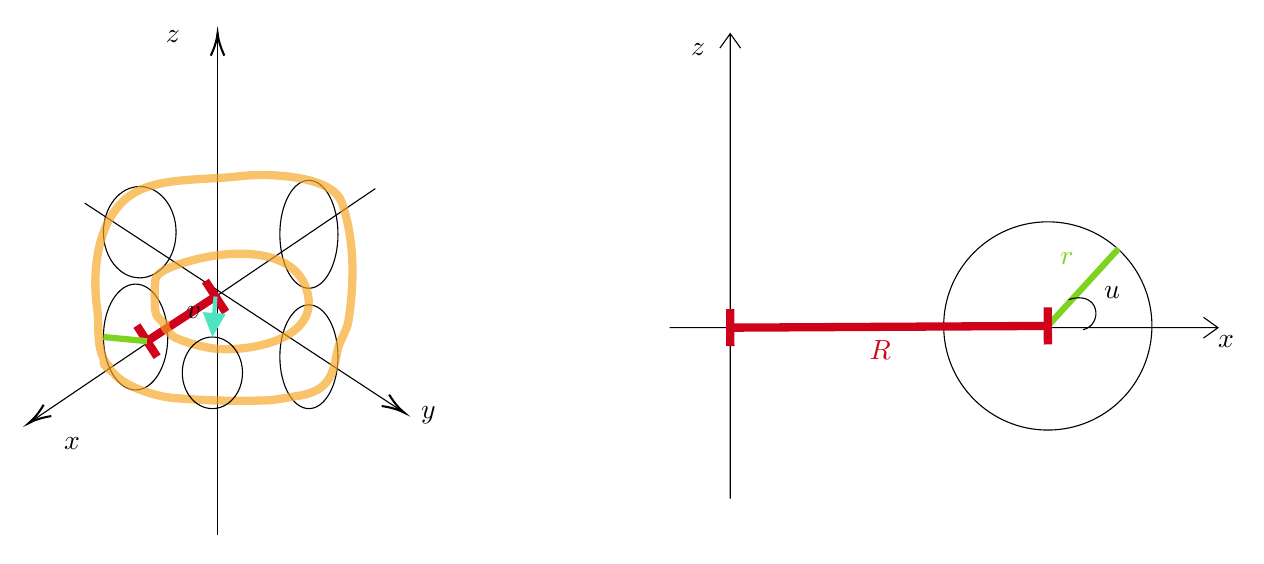
\begin{tikzpicture}[x=0.75pt,y=0.75pt,yscale=-1,xscale=1]
%uncomment if require: \path (0,300); %set diagram left start at 0, and has height of 300

%Shape: Axis 2D [id:dp7136936771401118] 
\draw  (340,176.67) -- (604.17,176.67)(369.17,35) -- (369.17,259) (597.17,171.67) -- (604.17,176.67) -- (597.17,181.67) (364.17,42) -- (369.17,35) -- (374.17,42)  ;
%Shape: Circle [id:dp5472771039380531] 
\draw   (472,175.83) .. controls (472,148.13) and (494.46,125.67) .. (522.17,125.67) .. controls (549.87,125.67) and (572.33,148.13) .. (572.33,175.83) .. controls (572.33,203.54) and (549.87,226) .. (522.17,226) .. controls (494.46,226) and (472,203.54) .. (472,175.83) -- cycle ;
%Straight Lines [id:da05831043255996615] 
\draw [color={rgb, 255:red, 126; green, 211; blue, 33 }  ,draw opacity=1 ][line width=2.25]    (522.17,175.83) -- (556.17,138.67) ;
%Curve Lines [id:da07142792001687193] 
\draw    (539.17,177.67) .. controls (549.17,175.17) and (547.17,158.17) .. (532.17,163.17) ;
%Straight Lines [id:da0764204193761383] 
\draw [color={rgb, 255:red, 208; green, 2; blue, 27 }  ,draw opacity=1 ][line width=3]    (369.17,176.67) -- (522.17,175.83) ;
\draw [shift={(522.17,175.83)}, rotate = 179.69] [color={rgb, 255:red, 208; green, 2; blue, 27 }  ,draw opacity=1 ][line width=3]    (0,8.94) -- (0,-8.94)   ;
\draw [shift={(369.17,176.67)}, rotate = 179.69] [color={rgb, 255:red, 208; green, 2; blue, 27 }  ,draw opacity=1 ][line width=3]    (0,8.94) -- (0,-8.94)   ;
%Straight Lines [id:da5252139346974255] 
\draw    (122.17,276.67) -- (122.17,36.67) ;
\draw [shift={(122.17,34.67)}, rotate = 90] [color={rgb, 255:red, 0; green, 0; blue, 0 }  ][line width=0.75]    (10.93,-3.29) .. controls (6.95,-1.4) and (3.31,-0.3) .. (0,0) .. controls (3.31,0.3) and (6.95,1.4) .. (10.93,3.29)   ;
%Straight Lines [id:da6118212643949656] 
\draw    (198.17,109.67) -- (32.82,221.55) ;
\draw [shift={(31.17,222.67)}, rotate = 325.92] [color={rgb, 255:red, 0; green, 0; blue, 0 }  ][line width=0.75]    (10.93,-3.29) .. controls (6.95,-1.4) and (3.31,-0.3) .. (0,0) .. controls (3.31,0.3) and (6.95,1.4) .. (10.93,3.29)   ;
%Straight Lines [id:da6992636664542036] 
\draw    (58.17,116.67) -- (210.49,216.57) ;
\draw [shift={(212.17,217.67)}, rotate = 213.26] [color={rgb, 255:red, 0; green, 0; blue, 0 }  ][line width=0.75]    (10.93,-3.29) .. controls (6.95,-1.4) and (3.31,-0.3) .. (0,0) .. controls (3.31,0.3) and (6.95,1.4) .. (10.93,3.29)   ;
%Shape: Ellipse [id:dp2918066307326016] 
\draw   (67.17,181.17) .. controls (67.17,167.08) and (74.11,155.67) .. (82.67,155.67) .. controls (91.23,155.67) and (98.17,167.08) .. (98.17,181.17) .. controls (98.17,195.25) and (91.23,206.67) .. (82.67,206.67) .. controls (74.11,206.67) and (67.17,195.25) .. (67.17,181.17) -- cycle ;
%Shape: Ellipse [id:dp8791248435789607] 
\draw   (152.17,190.67) .. controls (152.17,176.86) and (158.43,165.67) .. (166.17,165.67) .. controls (173.9,165.67) and (180.17,176.86) .. (180.17,190.67) .. controls (180.17,204.47) and (173.9,215.67) .. (166.17,215.67) .. controls (158.43,215.67) and (152.17,204.47) .. (152.17,190.67) -- cycle ;
%Shape: Ellipse [id:dp9198147198017402] 
\draw   (67.17,130.67) .. controls (67.17,118.52) and (75,108.67) .. (84.67,108.67) .. controls (94.33,108.67) and (102.17,118.52) .. (102.17,130.67) .. controls (102.17,142.82) and (94.33,152.67) .. (84.67,152.67) .. controls (75,152.67) and (67.17,142.82) .. (67.17,130.67) -- cycle ;
%Shape: Ellipse [id:dp23473871756026432] 
\draw   (152.17,131.67) .. controls (152.17,117.31) and (158.43,105.67) .. (166.17,105.67) .. controls (173.9,105.67) and (180.17,117.31) .. (180.17,131.67) .. controls (180.17,146.03) and (173.9,157.67) .. (166.17,157.67) .. controls (158.43,157.67) and (152.17,146.03) .. (152.17,131.67) -- cycle ;
%Straight Lines [id:da028711571087761567] 
\draw [color={rgb, 255:red, 208; green, 2; blue, 27 }  ,draw opacity=1 ][line width=3]    (121.17,161.67) -- (88.17,183.17) ;
\draw [shift={(88.17,183.17)}, rotate = 326.92] [color={rgb, 255:red, 208; green, 2; blue, 27 }  ,draw opacity=1 ][line width=3]    (0,8.94) -- (0,-8.94)   ;
\draw [shift={(121.17,161.67)}, rotate = 326.92] [color={rgb, 255:red, 208; green, 2; blue, 27 }  ,draw opacity=1 ][line width=3]    (0,8.94) -- (0,-8.94)   ;
%Straight Lines [id:da19483404785024994] 
\draw [color={rgb, 255:red, 126; green, 211; blue, 33 }  ,draw opacity=1 ][line width=2.25]    (88.17,183.17) -- (67.17,181.17) ;
%Shape: Free Drawing [id:dp7632615708303417] 
\draw  [color={rgb, 255:red, 245; green, 166; blue, 35 }  ,draw opacity=0.67 ][line width=3] [line join = round][line cap = round] (97.17,174.67) .. controls (94.3,174.67) and (99.53,180.54) .. (102.17,181.67) .. controls (107.56,183.98) and (114.13,185.91) .. (120.17,186.67) .. controls (136.43,188.7) and (172.35,182.61) .. (165.17,158.67) .. controls (158.9,137.79) and (129.04,139.45) .. (112.17,143.67) .. controls (107.21,144.9) and (92.51,148.56) .. (92.17,153.67) .. controls (91.83,158.66) and (91.64,163.69) .. (92.17,168.67) .. controls (92.6,172.74) and (97.17,173.92) .. (97.17,176.67) ;
%Shape: Free Drawing [id:dp4934917235667049] 
\draw  [color={rgb, 255:red, 245; green, 166; blue, 35 }  ,draw opacity=0.67 ][line width=3] [line join = round][line cap = round] (70.17,195.67) .. controls (62.93,188.43) and (65.46,176.74) .. (64.17,167.67) .. controls (61.13,146.41) and (65.21,118.05) .. (86.17,109.67) .. controls (99.39,104.38) and (118.81,105.46) .. (133.17,103.67) .. controls (144.08,102.3) and (177.47,102.58) .. (182.17,116.67) .. controls (188.29,135.03) and (188.12,154.45) .. (185.17,173.67) .. controls (184.54,177.77) and (180.76,183.72) .. (180.17,186.67) .. controls (177.8,198.51) and (176.83,207.29) .. (160.17,209.67) .. controls (155.93,210.27) and (150.22,211.53) .. (146.17,211.67) .. controls (137.17,211.98) and (128.16,211.98) .. (119.17,211.67) .. controls (113.49,211.47) and (107.83,211) .. (102.17,210.67) .. controls (93.12,210.13) and (77.44,205.26) .. (72.17,198.67) .. controls (71.45,197.77) and (67.17,195.01) .. (67.17,193.67) ;
%Shape: Ellipse [id:dp24103730137849944] 
\draw   (105.17,198.42) .. controls (105.17,188.89) and (111.66,181.17) .. (119.67,181.17) .. controls (127.67,181.17) and (134.17,188.89) .. (134.17,198.42) .. controls (134.17,207.94) and (127.67,215.67) .. (119.67,215.67) .. controls (111.66,215.67) and (105.17,207.94) .. (105.17,198.42) -- cycle ;
%Straight Lines [id:da31558128568600174] 
\draw [color={rgb, 255:red, 80; green, 227; blue, 194 }  ,draw opacity=1 ][line width=1.5]    (121.17,161.67) -- (119.97,177.18) ;
\draw [shift={(119.67,181.17)}, rotate = 274.4] [fill={rgb, 255:red, 80; green, 227; blue, 194 }  ,fill opacity=1 ][line width=0.08]  [draw opacity=0] (11.61,-5.58) -- (0,0) -- (11.61,5.58) -- cycle    ;

% Text Node
\draw (349,38.4) node [anchor=north west][inner sep=0.75pt]    {$z$};
% Text Node
\draw (603,179.4) node [anchor=north west][inner sep=0.75pt]    {$x$};
% Text Node
\draw (548,155.4) node [anchor=north west][inner sep=0.75pt]    {$u$};
% Text Node
\draw (435,181.4) node [anchor=north west][inner sep=0.75pt]  [color={rgb, 255:red, 208; green, 2; blue, 27 }  ,opacity=1 ]  {$R$};
% Text Node
\draw (527,139.4) node [anchor=north west][inner sep=0.75pt]  [color={rgb, 255:red, 126; green, 211; blue, 33 }  ,opacity=1 ]  {$r$};
% Text Node
\draw (96,32.4) node [anchor=north west][inner sep=0.75pt]    {$z$};
% Text Node
\draw (219,213.4) node [anchor=north west][inner sep=0.75pt]    {$y$};
% Text Node
\draw (47,228.4) node [anchor=north west][inner sep=0.75pt]    {$x$};
% Text Node
\draw (106,165.4) node [anchor=north west][inner sep=0.75pt]    {$v$};


\end{tikzpicture}



Let $u$ represent this new ``$\phi$"and $v$ represent $\theta$.

If we have our $u$ go from the $xy$-plane, we can reach all parts of donut from $u =0$ to $u =2\pi$.

We're going around the entire donut, so our bounds for $v$ are $v=0$ and $v=2\pi$.


In this new ``spherical coordinate" system,
\begin{align*}
    x&=r\cos v\tag{$r=\rho\cos u$}\\
    y&=r\sin v\tag{$r=\rho\cos u$}\\
    z&=\rho\sin u
\end{align*}
We need to account for that fact that the circle has radius $r$ and center $(R,0,0)$. Based on my amazing drawings,
\begin{align*}
    x&=(R+r\cos u)\cos v\\
    y&=\lrp{R+r\cos u}\sin v\\
    z&=r\sin u
\end{align*}
Therefore, our parametrization is
\begin{equation*}
    \r(u,v)=\lra{(R+r\cos u)\cos v, (R+r\cos u)\sin v, r\sin u}\tag{$0\leq u\leq 2\pi$, $0\leq v\leq 2\pi$}
\end{equation*}
\phantomsection
\addcontentsline{toc}{subsection}{Surface Area}\textbf{Surface Area}

Now that we have our parameterization, let's calculate the surface area.

Recall that the surface area is
\begin{align*}
    S&=\iint_R \norm{\frac{\partial \r}{\partial u}\times \frac{\partial \r}{\partial v}}\,dA
\end{align*}
We know our region is $0\leq u\leq 2\pi$ and $0\leq v\leq 2\pi$.

Let's find what $\displaystyle\norm{\frac{\partial \r}{\partial u}\times \frac{\partial \r}{\partial v}} $ is.

Since $\displaystyle \r(u,v)=\lra{(R+r\cos u)\cos v, (R+r\cos u)\sin v, r\sin u}$,
\begin{align*}
    \frac{\partial \r}{\partial u}&=\lra{-r\sin u\cos v, -r\sin u\sin v, r\cos u}\\
    \frac{\partial \r}{\partial v}&=\lra{-\lrp{R+r\cos u}\sin v, \lrp{R+r\cos u}\cos v, 0}\\
    \frac{\partial \r}{\partial u}\times \frac{\partial \r}{\partial }&=\begin{vmatrix}
    \i & \j &\k\\
    -r\sin u\cos v& -r\sin u\sin v & r\cos u\\
    -(R+r\cos u)\sin v & \lrp{R+r\cos u}\cos v&0
    \end{vmatrix}\\
    &=\lrp{\lrp{R+r\cos u}\lrp{r\cos u \cos v}}\i -\lrp{\lrp{R+r\cos u}\lrp{r\cos u \sin v}}\j + \lrp{\lrp{R+r\cos u}\lrp{-r\sin u}}\k\tag{please PM me if needed}\\
    &=\lra{\lrp{R+r\cos u}\lrp{r\cos u \cos v},-{\lrp{R+r\cos u}\lrp{r\cos u \sin v}},\lrp{R+r\cos u}\lrp{-r\sin u}}\\
    \norm{\frac{\partial \r}{\partial \phi}\times \frac{\partial \r}{\partial \theta}}&=\sqrt{(R+r\cos u)^2(r^2\cos^2 u \cos^2 v)+(R+r\cos u)^2(r^2\cos^2 u \sin^2 v)+(R+r\cos u)^2(r^2\sin^2u)}\\
    &=\sqrt{(R+r\cos u)^2(r^2\cos^2u)\lrp{\cos^2 v+\sin^2 v}+(R+r\cos u)^2\lrp{r^2\sin^2 u}}\\
    &=\sqrt{(R+r\cos u)^2(r^2\cos ^2 u)+(R+r\cos u)^2(r^2\sin^2 u)}\tag{$\cos^2 v+\sin^2 v=1$}\\
    &=\sqrt{(R+r\cos u)^2(r^2)(\cos^2 u +\sin^2 u)}\\
    &=\sqrt{(R+r\cos u)^2(r^2)}\tag{$\cos ^2 u+\sin^2 u=1$}\\
    &=(R+r\cos u)(r)\\
    &=Rr+r^2\cos u
\end{align*}
Let's evaluate the integral.
\begin{align*}
    S&=\int_0^{2\pi}\int_0^{2\pi}Rr+r^2\cos u\,du\,dv\\
    &=\int_0^{2\pi}\lrb{Rru+r^2\sin u}_0^{2\pi}\,dv\\
    &=\int_0^{2\pi} \lrp{2Rr\pi + 4\pi^2\sin 2\pi}-\lrp{0+0}\,dv\\
    &=\int_0^{2\pi} 2Rr\pi\,dv\tag{$\sin2\pi=0$}\\
    &=\lrb{2Rr\pi v}_0^{2\pi}\\
    &=2Rr\pi\lrp{2\pi}\\
    &=4 Rr\pi^2\\
    &=4\pi^2Rr
\end{align*}
\newpage
\phantomsection
\addcontentsline{toc}{section}{Problem 4}\textbf{Problem 4}


Use spherical coordinates to write a parametrization of the ellipsoid
\begin{equation*}
    \frac{x^2}{a^2}+\frac{y^2}{b^2}+\frac{z^2}{c^2}=1
\end{equation*}
Then set up an integral to find the surface area.

\Solution

\phantomsection
\addcontentsline{toc}{subsection}{Parametrization}\textbf{Parametrization}

Let's (kind of) use spherical coordinates!

Recall that in spherical coordinates,
\begin{align*}
    x&=\rho \sin \phi\cos\theta\\
    y&=\rho \sin \phi\sin\theta\\
    z&=\rho \cos\phi
\end{align*}
Like with Problem 3, we might not want to have our angle $\phi$ start at the ``north pole" (pos $z$-axis). Instead, let's start our ``$\phi$" from the $xy$-plane. We can have $\psi =\dfrac{\pi}{2}-\phi$ be our new $\phi$. We can keep $\theta$ the same as it was with spherical coordinates.




\tikzset{every picture/.style={line width=0.75pt}} %set default line width to 0.75pt        

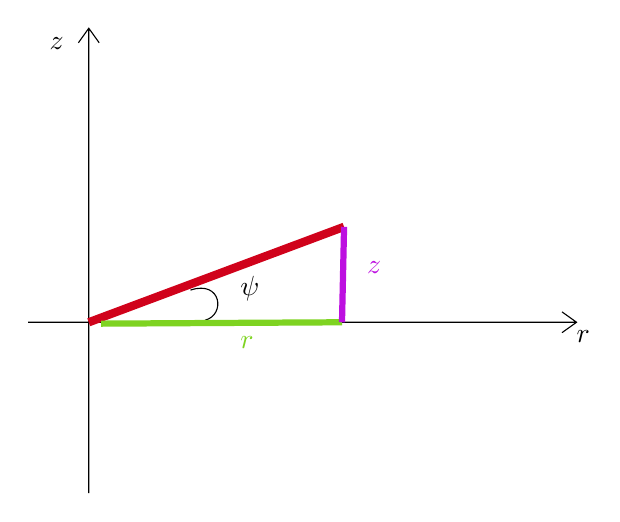
\begin{tikzpicture}[x=0.75pt,y=0.75pt,yscale=-1,xscale=1]
%uncomment if require: \path (0,300); %set diagram left start at 0, and has height of 300

%Shape: Axis 2D [id:dp3868879526535256] 
\draw  (212,174.67) -- (476.17,174.67)(241.17,33) -- (241.17,257) (469.17,169.67) -- (476.17,174.67) -- (469.17,179.67) (236.17,40) -- (241.17,33) -- (246.17,40)  ;
%Curve Lines [id:da7616688363692427] 
\draw    (297.17,173.67) .. controls (307.17,171.17) and (305.17,154.17) .. (290.17,159.17) ;
%Straight Lines [id:da9959122238211519] 
\draw [color={rgb, 255:red, 208; green, 2; blue, 27 }  ,draw opacity=1 ][line width=3]    (241.17,174.67) -- (364.17,128.67) ;
%Straight Lines [id:da8585096856285587] 
\draw [color={rgb, 255:red, 126; green, 211; blue, 33 }  ,draw opacity=1 ][line width=2.25]    (247.17,175.33) -- (363.17,174.67) ;
%Straight Lines [id:da05876942804651064] 
\draw [color={rgb, 255:red, 189; green, 16; blue, 224 }  ,draw opacity=1 ][line width=2.25]    (364.17,128.67) -- (363.17,174.67) ;

% Text Node
\draw (221,36.4) node [anchor=north west][inner sep=0.75pt]    {$z$};
% Text Node
\draw (475,177.4) node [anchor=north west][inner sep=0.75pt]    {$r$};
% Text Node
\draw (313,151.4) node [anchor=north west][inner sep=0.75pt]    {$\psi $};
% Text Node
\draw (313,180.4) node [anchor=north west][inner sep=0.75pt]  [color={rgb, 255:red, 126; green, 211; blue, 33 }  ,opacity=1 ]  {$r$};
% Text Node
\draw (374,144.4) node [anchor=north west][inner sep=0.75pt]  [color={rgb, 255:red, 189; green, 16; blue, 224 }  ,opacity=1 ]  {$z$};


\end{tikzpicture}



With this new change we now get
\begin{align*}
    x&=\rho\cos\psi\cos\theta\tag{now, $r=\rho\cos\psi$}\\
    y&=\rho\cos\psi\sin\theta\tag{now, $r=\rho\cos\psi$}\\
    z&=\rho\sin\psi
\end{align*}
We just need to figure out what $\rho$ is in each of our coordinates (it's not necessarily going to be the same since this is an ellipsoid with $a$, $b$, and $c$).

Since
\begin{equation*}
    \frac{x^2}{a^2}+\frac{y^2}{b^2}+\frac{z^2}{c^2}=1
\end{equation*}
Let's have $\rho=a$ for $x$, $\rho=b$ for $y$, and $\rho =c$ for $z$.

If these substitutions are correct, we should get
\begin{equation*}
    \frac{x^2}{a^2}+\frac{y^2}{b^2}+\frac{z^2}{c^2}=1
\end{equation*}
in our ellipsoid equation.

Let's check if this is the case.
\begin{align*}
    \frac{(a\cos\psi\cos\theta)^2}{a^2}+\frac{(b\cos\psi\sin\theta)^2}{b^2}+\frac{(c\sin\psi)^2}{c^2}&=\frac{a^2\cos^2\psi\cos^2\theta}{a^2}+\frac{b^2\cos^2\psi\sin^2\theta}{b^2}+\frac{c^2\sin^2\psi}{c^2}\\
    &=\cos^2\psi\cos^2\theta+\cos^2\psi\sin^2\theta+\sin^2\psi\\
    &=\cos^2\psi\lrp{\cos^2\theta+\sin^2\theta}+\sin^2\psi\\
    &=\cos^2\psi+\sin^2\psi\tag{$\cos^2\theta+\sin^2\theta=1$}\\
    &=1\tag{$\cos^2\psi+\sin^2\psi=1$}
\end{align*}
Since 
\begin{equation*}
    \frac{x^2}{a^2}+\frac{y^2}{b^2}+\frac{z^2}{c^2}=1
\end{equation*}
where $x=a\cos\psi\cos\theta$, $y=b\cos\psi\sin\theta$, and $z=c\sin\psi$, our parameterization is correct.

Let's find the bounds for $\psi$ and $\theta$.

For $u$,

If we look at the ellipsoid from the ``front view", we'll notice that $\psi$ goes from $\psi=0$ to $\psi=2\pi$ to cover the entire ellipsoid.

This is a generic graph of an ellipsoid.
\begin{center}
\resizebox{5cm}{!}{
    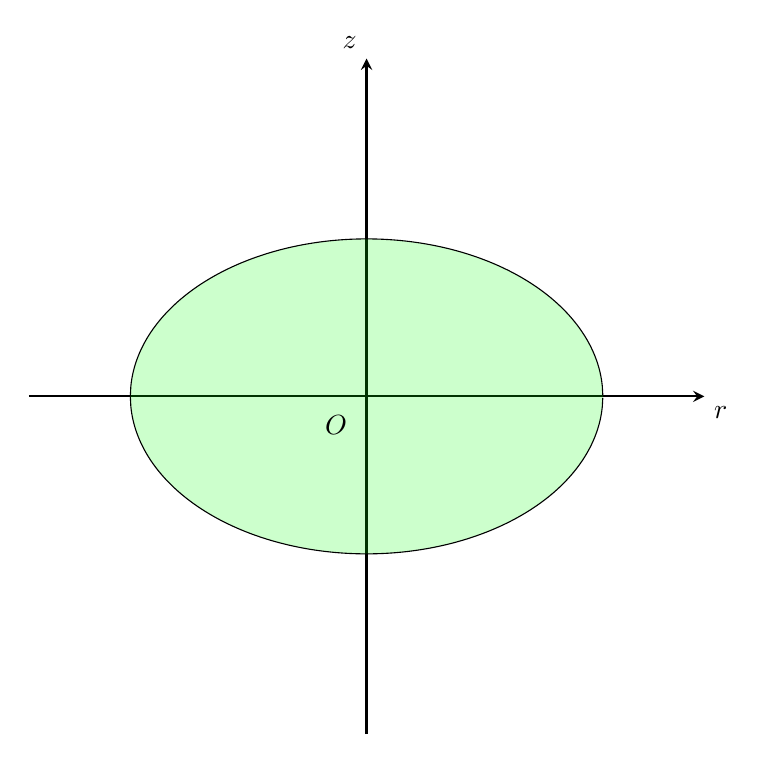
\begin{tikzpicture}
    \begin{axis}[standard,
            xtick={-10,10},
            ytick={-10,10},
            samples=1000,
            xlabel={$r$},
            ylabel={$z$},
            xmin=-3.3,xmax=3.3,
            ymin=-3.3,ymax=3.3,
            x=1cm,
            y=1cm/1,
            x
           ]
\node[anchor=center,label=south west:$O$] at (axis cs:0,0){};
\addplot[name path=F,domain={-3:3}]{sqrt(4-(4/9)*x^2)};
\addplot[name path=G,domain={-3:3}]{-sqrt(4-(4/9)*x^2)};
\addplot[fill=green, fill opacity=0.2] fill between [of=F and G, soft clip={domain=-3:3}];
    \end{axis}
    \end{tikzpicture}
}
\end{center}

For $v$,

If we look at the ellipsoid from the ``top view", we'll notice that $\theta$ goes from $\theta=0$ to $\theta=2\pi$ to cover the entire ellipsoid.

This is a generic graph of an ellipsoid.
\begin{center}
\resizebox{5cm}{!}{
    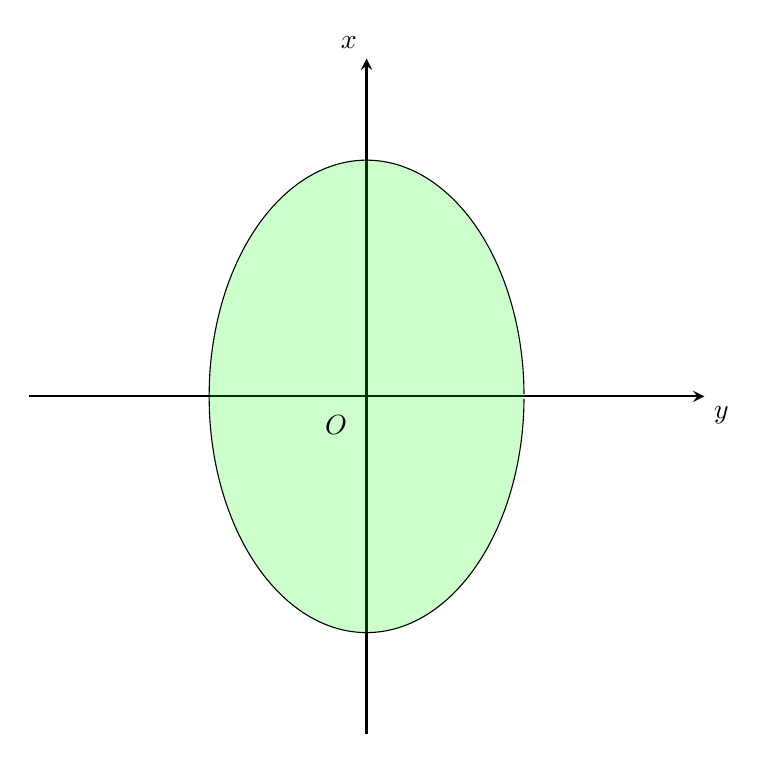
\begin{tikzpicture}
    \begin{axis}[standard,
            xtick={-10,10},
            ytick={-10,10},
            samples=1000,
            xlabel={$y$},
            ylabel={$x$},
            xmin=-3.3,xmax=3.3,
            ymin=-3.3,ymax=3.3,
            x=1cm,
            y=1cm/1,
            x
           ]
\node[anchor=center,label=south west:$O$] at (axis cs:0,0){};
\addplot[name path=F,domain={-2:2}]{sqrt(9-(9/4)*x^2)};
\addplot[name path=G,domain={-2:2}]{-sqrt(9-(9/4)*x^2)};
\addplot[fill=green, fill opacity=0.2] fill between [of=F and G, soft clip={domain=-2:2}];
    \end{axis}
    \end{tikzpicture}
}
\end{center}
Since we're going around the entire ellipsoid, $0\leq \theta\leq 2\pi$.

Therefore, our bounds are $0\leq \psi\leq 2\pi$ and $0\leq \theta\leq 2\pi$.

Our parameterization is
\begin{equation*}
    \r(\phi,\theta)=\lra{a\cos \psi\cos \theta, b\cos \psi\sin \theta c\sin \psi}\tag{$0\leq \psi\leq 2\pi$, $0\leq \theta\leq 2\pi$}
\end{equation*}
\phantomsection
\addcontentsline{toc}{subsection}{Surface Area}\textbf{Surface Area}

Now that we have our parameterization, let's calculate the surface area.

Recall that the surface area is
\begin{align*}
    S&=\iint_R \norm{\frac{\partial \r}{\partial u}\times \frac{\partial \r}{\partial v}}\,dA
\end{align*}
Let $u=\phi$ and $v=\theta$.

We know our region is $0\leq \phi\leq 2\pi$ and $0\leq \theta\leq 2\pi$.

Let's find what $\displaystyle\norm{\frac{\partial \r}{\partial \psi}\times \frac{\partial \r}{\partial \theta}} $ is.

Since $\displaystyle \r(u,v)=\lra{a\cos \psi\cos \theta, b\cos \psi\sin \theta c\sin \psi}$,
\begin{align*}
    \frac{\partial \r}{\partial \psi}&=\lra{-a\sin \psi\cos \theta, -b\sin \psi\sin\theta, c\cos \psi}\\
    \frac{\partial \r}{\partial \theta}&=\lra{-a\cos\psi\sin\theta, b\cos\psi\cos\theta, 0}\\
    \frac{\partial \r}{\partial \psi}\times \frac{\partial \r}{\partial \theta}&=\begin{vmatrix}
    \i & \j & \k\\
    -a\sin \psi\cos \theta &-b\sin \psi\sin\theta &c\cos \psi\\
    -a\cos\psi\sin\theta&b\cos\psi\cos\theta&0
    \end{vmatrix}\\
    &=\lrp{0-bc\cos^2\psi\cos\theta}\i -\lrp{0+ac\cos^2\psi\sin\theta}\j+\lrp{-ab\sin\psi\cos\psi\cos^2\theta-ab\sin\psi\cos\psi\sin^2\theta}\k\\
    &=\lrp{-bc\cos^2\psi\cos\theta}\i-\lrp{ac\cos^2\psi\sin\theta}\j+\lrp{-ab\sin\psi\cos\psi\lrp{\cos^2\theta+\sin^2\theta}}\k\\
    &=\lrp{-bc\cos^2\psi\cos\theta}\i-\lrp{ac\cos^2\psi\sin\theta}\j+\lrp{-ab\sin\psi\cos\psi}\k\tag{$\cos^2\theta+\sin^2\theta=1$}\\
    \norm{\frac{\partial \r}{\partial \psi}\times \frac{\partial \r}{\partial \theta}}&=\sqrt{\lrp{-bc\cos^2\psi\cos\theta}^2+\lrp{ac\cos^2\psi\sin\theta}^2+\lrp{-ab\sin\psi\cos\psi}^2}\\
    &=\sqrt{b^2c^2\cos^4\psi\cos^2\theta+a^2c^2\cos^4\psi\sin^2\theta+a^2b^2\sin^2\psi\cos^2\psi}
\end{align*}
No further simplification can be done.

Our surface area integral must be
\begin{align*}
    S&=\int_0^{2\pi}\int_0^{2\pi}\sqrt{b^2c^2\cos^4\psi\cos^2\theta+a^2c^2\cos^4\psi\sin^2\theta+a^2b^2\sin^2\psi\cos^2\psi}\,d\psi\,d\theta
\end{align*}
\end{document}
